\documentclass[a4paper, 11pt, notitlepage]{report}

\usepackage{amsfonts} % if you want blackboard bold symbols e.g. for real numbers
\usepackage{graphicx} % if you want to include jpeg or pdf pictures
\usepackage{geometry}
\usepackage{amsmath}
\usepackage[hidelinks]{hyperref}
\usepackage[official]{eurosym}
\setcounter{secnumdepth}{5}

\title{{\Huge Modelling Project} \vspace{290pt}} % change this
\author{Yoram Meijaard - y.j.meijaard@student.tue.nl\\Chiel van Horssen - c.v.horssen@student.tue.nl\\Youri Haenen - y.h.b.haenen@student.tue.nl\\Bram Maas - b.j.g.maas@student.tue.nl\\Martijn Ras - n.m.j.ras@student.tue.nl} % change this
\date{Due to April 5 2015} % change this

\begin{document}

%%%%%%%%%% PRELIMINARY MATERIAL %%%%%%%%%%
\maketitle
\begin{center}
The report on the wheelchair problem of airline companies % change this
\\[12pt]
Supervised by: I. Papaliouras \\ Assessor: J. Nederhof % change this
\\[12pt]
This document contains 3 appendices.
\end{center}
\thispagestyle{empty}
\newpage


\tableofcontents

%%%%%%%%%% MAIN TEXT STARTS HERE %%%%%%%%%%

%Hand-in date;  deadline

%Number of attachments; Appendices

%%%%%%%%%% SAMPLE CHAPTER %%%%%%%%%%
% \chapter{Summary}

% \chapter{Description of modeling process}


\setcounter{chapter}{+5}
\chapter{Context}
\section{The Stakeholders and the keydrivers }
The stakeholders are:
\begin{itemize}
 \item KLM
 \item Escorts
 \item Passengers
 \item Employees
 \item Other airline companies and other airport
 \item  constructors and maintainers of the wheelchairs.
\end{itemize}
These person have got the greatest interest in the escort service in general, including if the service was optimized to be efficient in time and thus in costs. The people who guard the depot where the wheelchairs are stored and desk workers who check in the passengers are both taken into account in the employees. The keydrivers are:
\begin{itemize}
	\item Efficiency
	\item Cost
	\item Optimization
	\item Comfort
	\item Time
	\item Safety
	\item Reliability
\end{itemize}
\section{Relation between the stakeholders and keydrivers}
If the Stakeholders are linked to the keydrivers, their relations could be summarized into this mind map:
\begin{center}
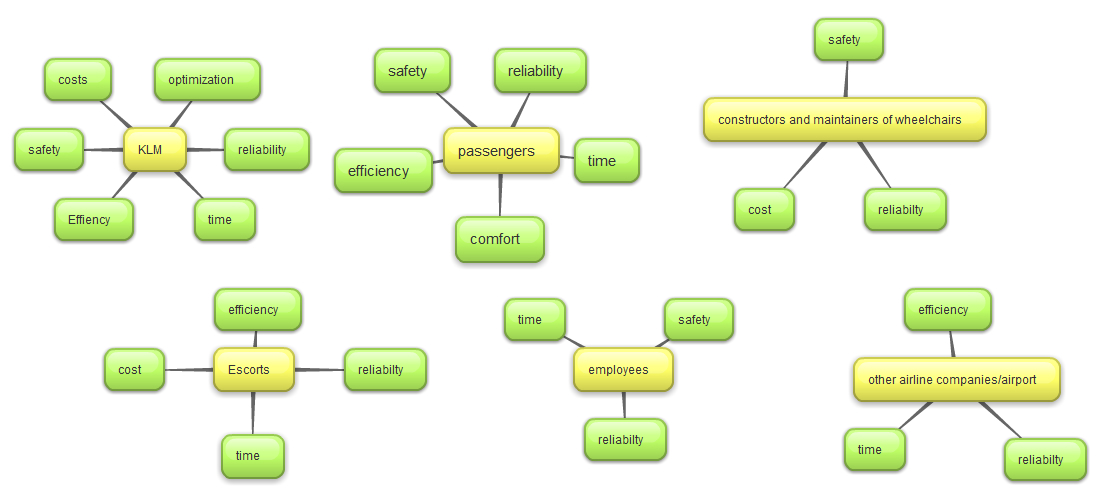
\includegraphics[scale=0.4]{figures/relationstakeholders.jpg}
\end{center}
\subsection{KLM}
One of the interests of KLM is the costs to keep them as low as possible, but not such that this is the main interest. The plane needs to leave on time, so there needs to be a minimum amount of money to realize the on time depart of the plane.\\
Safety is another interest, which deals with the safety of the escort service. This deals then with the safety of the trip, the safety of the wheelchairs etc. If the safety is not of a certain level, such that the reputation of the airline company suffers, people might rather use other airline companies to realize their trip.\\
The same reason holds for efficiency. Also, if the service is not efficient, not as many escorts by the same person can be taken care of, so the plane might leave late. Therefore an efficient solution with respect to time needs to be archived.\\
So as mentioned above, time is also a factor which is required to keep costs low and hence a high efficiency as result. The distance from the check-in desk to the gate can be considered in time for example.\\
Reliability of the service also deals with the safety reasons: KLM needs to be sure the service takes a certain time and it should be sure that the passengers arrive on time at the gate. Unreliable service leads to loss of money and reputation damage.\\
Finally, optimization is the most important interest for KLM, so the service gets optimized to cost minimally but that the plane can depart on time.
\subsection{Escorts}
The costs are also important for the escort itself. If the costs are getting too high, the might be a possibility that these people are fired or a drop in wage. So indirectly they have an interest in the costs of their service.\\
With respect to the efficiency, which is also a keydriver for the escorts, time is important. This relates to the costs (as mentioned above), because the more escorts executed, the more employees are required to perform all escorts, which means higher costs, hence in contradiction with the main goal. \\
Reliability is required by the escort, such KLM can assure the passengers that they will be on time at the gate, so again also to keep costs low. On the other hand, other personnel of the service needs to be sure that certain staff is at position x at time t, so efficiently using the resources and personnel of the service to optimize the service.\\
Efficiency follows then directly from the above mentioned relations in order to keep costs low of the service.
\subsection{Passengers}
The passengers are interested in having a comfortable, safe, efficient and reliable escort. Comfort can be archived by having a sufficient comfortable ride and wheelchair used to transport the person from the desk to the gate. Since the passenger does not want to see the whole airport,  time is also in the interest of the passengers. This also relates to efficiency: the disabled passenger wants to be escorted in the shortest possible time, with as much comfort as possible. This means that some  is required and hence the service needs to be efficient. \\
The reliability is of interest for the passengers, by the fact that
the passenger wants to be sure to get the escort when request, which in generally happens. Also, the passenger want to be brought to a specific gate, at a specific time. Therefore the reliability of the escort service is also of interest for the passengers.\\
Finally, safety is also of interest, because the passenger wants to be escorted safely without injuries. Therefore the wheelchair needs to be safe to be used, and the quality of service of the escort needs to be of a certain level. This level requires a certain level of service from the personnel.
\subsection{Employees}
The interest of the employees, are the time (duration of the escort), reliability and the safety of the escort. The time is of interest, because of the fact that when a transfer has to be made, the escort is on time at the gate to get the passenger and is on time at the next gate to board the passenger such that the next plane (also) can leave on time. The employees guarding the depot on the other hand have got an interest in time as well. Their interest is to know how long a wheelchair is away from the depot, but also to be able to check if something happened with the escort or the wheelchair (i.e. lost or accident). \\
Safety is also of concerns of the employees, since if the goal of an airline company is to maintain quality and safety, all employees should be able to contribute in their way. The escorting persons therefore need to make sure the escorted person is moved safely from place A to place B.
\subsection{Constructors and maintainers of the wheelchairs}
The maintainers and constructors of the wheelchairs have interest in the safety, costs and reliability. They have to make sure the wheelchair is safe,  in usage for both the disabled person and the escort service. The escort service could get a bad reputation if the escort service is not safe.\\
On the other hand, the costs should not be too high. So the people have to construct and maintain the wheelchairs in such a way to create good wheelchairs with not too high costs (both maintenance and product price). But the demand for low costs is opposed by the safety of the wheelchairs. If the construction is not solid enough so any\footnote{Obviously not everyone should be taken into account, but i.e. obese people need tougher wheelchairs, hence some 'extremes' need to be taken care of in the construction, but not all.} possible disabled person can be transferred safely. So the wheelchair also needs to be sufficiently solid built.
\subsection{Other airline companies and other airports}
Other airline companies and other airports also have an interest in the escort service in the following perspective. If the transfer is a transfer between two different planes of different airline companies\footnote{Only from KLM to airline company X is considered}, the other company requiers a time efficient, reliable escort service such that this plane can depart on time.\\
In the worst case, there is little time between arrival of plane 1 and depart of plane 2. A time efficient service would be necessary to realize this. Also an estimation on when a disables person with escort arrives is pleasant to know when an escort approximately arrives. Clearly, this should be as efficient as possible and hence efficiency is also an interest.\\
Reliability is also an interest for other airline companies and airports. Being sure when an escort arrives is necessary in order to make it possible for other airline companies to depart on time when there is a transfer with escort service. If it is uncertain if the passenger will arrive on time, it is cheaper for an airline company to let the plane depart and put the escorted person on a plane departing later than to miss the timeslot in which the plane was supposed to leave with all (worse) economic consequences as result. Therefore reliability of the escort service is also of interest for other airports and other airline companies.
\newpage
\section{Relation between keydrivers}
The keydrivers do also have a relation with other keydrivers than only with stakeholders. These can be summarized as follows:
\begin{center}
	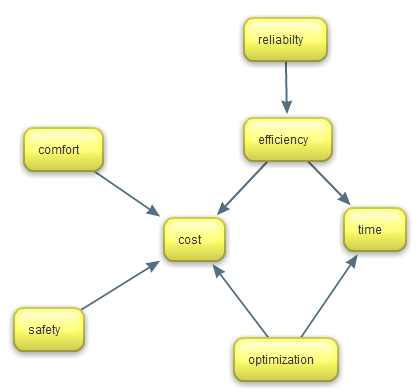
\includegraphics[scale=0.45]{figures/relationkeydrivers.jpg}
\end{center}
The arrows should be read that keydriver $k$ has in incoming arrow from $k'$, and $k'$ has and incoming arrow from $k"$, $k$ is in a relation with $k"$. So there is transitivity between the elements.
\subsection{Reliability}
In order to have a reliable service, so the service is on time and there are no losses of money on the service, it can be said that reliability is linked to both cost and time in the respect of efficiency. Therefore by transitivity reliability is related to efficiency.
\subsection{Efficiency}
As stated by reliability, the costs should not be low and the escort should be time efficient. So in general the service needs to be both efficient in time and costs. Therefore efficiency has a relation with both cost and time.
\subsection{Optimization}
So both time and cost should be in relation with optimization. The cost should be kept as low as possible to give an time efficient reliable service. But then there should be optimization on time with costs reduction as a result\footnote{Compared to the case where no attention has been paid to optimized model where planes leave late with all financial consequences as result}. Therefore there needs to be a relation from optimization to both cost and time.
\subsection{Safety}
When safety is addressed, money is always a factor. Safety costs money, and the level of safety sets the costs in order to realize. If for example the wheelchair needs to be made that it has bumpers to take the impact and not the one sitting in the wheelchair. But this costs money to realize. This shows the direct relation between safety and cost, which therefore exists.
\subsection{Comfort}
The comfort also relates to money in the same respect as safety does. If the transported person is transported in a very relaxing wheelchair, then this wheelchair costs more money than a plain wheelchair. If the ride to the gate is desired to be more comfortable, then the duration needs to be longer which as a result costs more money. Hence, comfort is in a relation with cost.
%%%%%%%%%%%%%%%%%%%%%%%%%%%%%%%%%%%%%%%%%%%%%%%%%%%%%%%%%%%%%%%%%%%%%%%%%%%%%%%%%%%%%%%%
\chapter{Problem definition and purpose}
\section{Model purpose}
When making a model there should be three questions answered:\\
\emph{Is there something to choose?\\
Will the model output a number?\\
Should the model produce a value or knowledge?}\\\\
The first question can be answered with \emph{yes}, that is because there are different combinations for different sets of people, area etc.\\
The second question will also be answered with \emph{yes} since the model should produce a number of escorts or wheelchairs needed so the cost can be calculated.\\
The answer to the last question should be a \emph{value}, because the model brings an optimized solution rather than new knowlage.\\ From this we can conclude the model should be a \emph{optimization}, it should produce the best solution possible for the owner.
\section{Model dimensions}
Now that the purpose of the model is known, the dimensions should be determined. This can be done using the following points.
\subsection{Continue or discrete}
The model should be a \emph{discrete} model, since both input and output values will be both integers (real life objects like number of wheelchairs, escorts) and floats (salary, costs). Also most of the intermediate results will be discrete numbers.
\subsection{Deterministic or stochastic}
Since the owner of the model can decide almost all input variables, the assumption is that this model is \emph{deterministic}. The owner has influence on most of the inputs, and also the number of wheelchairs and disabled people will be deterministic.
\subsection{Black box or glass box}
The model will be a \emph{glass box} model, because there is insight in what happens, everything is known by the owner of the model, for instance the owner knows how many disabled people travel and where and when planes arrive and leave.
\subsection{Static or dynamic}
Because time does not matter -the model is, after all, just about one transfer- this is a \emph{static} model. All input values are set before execution and are valid throughout the entire model.
\subsection{Calculating or reasoning}
The model will be a \emph{calculating} model, because a number is the desired output of the model. Also all input values and quantities will be numbers.
\subsection{Geometrical or non-geometrical}
Even though an airport feels like a geometric setting the model is a \emph{non-geometrical} model, this is because the airport will not be geographically defined, there are only distances used which are abstract numbers.
\subsection{Numerical or symbolic}
It is not entirely clear whether the model is numerical or symbolic since the model itself starts out using only symbols for the inputs in the formulas, but once executed the the model will replace these with concrete values, also the output will be numerical. This makes the model \emph{both numerical and symbolic}.
\subsection{Material or immaterial}
The model will be \emph{Immaterial}, because the model does not describe a real airport. There is just a concept in our mind that we project into this immaterial model. It will sort of look like modeling from scratch, but with a discrete model.
\section{Conceptual definition of the problem}
Given a description of the airport, incoming flights and departing flights: how many resources are required to get a flight of the ground in time with all disabled people on board?
\chapter{Sub-questions}
\begin{enumerate}
\item How will the number of wheelchairs influence the amount of time of a transfer between two flights?
\item How will the location of the wheelchair depot influence the time?
	\begin{enumerate}
	\item What will this mean for the distance between the gates?
	\item What will this mean for the time required to travel between to gates?
	\item What will this mean for the maintenance of the wheelchairs
		\begin{enumerate}
		\item Who will do the maintenance of the wheelchairs?
		\item How much service does each wheelchair require?
		\item Where will those wheelchairs be bought?
		\end{enumerate}
	\item How will this influence the amount of escorts?
		\begin{enumerate}
		\item How many escorts do I need for one wheelchair?
		\end{enumerate}
	\item Will the storing of the chairs at one location decrease the costs of guarding them?
		\begin{enumerate}
		\item Will hiring additional security to guard the wheelchairs result in less damage/stolen chairs?
		\item If the escorts guard the chairs, how will this influence security?
			\begin{enumerate}
			\item Do we have to hire more escorts if they handle security?
			\end{enumerate}
		\end{enumerate}
	
	\end{enumerate}
\item What kind of wheelchairs will be used?
	\begin{enumerate}
	\item Will the quality of the chair influence the amount of maintenance required?
	\item Will the quality of the chair influence the amount of money asked for the service?
	\item How will the quality of the wheelchair influence the customer satisfaction?
		\begin{enumerate}
		\item How will this distinct KLM from other airliners?
		\item Will this create an increase in customers?
		\end{enumerate}
	\item Which wheelchair has the best price/quality rate?
		\begin{enumerate}
		\item How much is the difference in price?
			\begin{enumerate}
			\item How will the difference in price influence the total costs?
			\item What is the price of each wheelchair?
			\end{enumerate}
		\end{enumerate}
	\end{enumerate}
\item How will the amount of escorts influence the total costs?
	\begin{enumerate}
	\item What kind of people will escort the disabled?
		\begin{enumerate}
		\item Will the use of students influence the amount of customers that want to use the service?
		\item Will the use of athletes influence the average travel speed of an wheelchair?
		\item What kind of education/degree do they need?

		\end{enumerate}
	\item How much will the escorts be paid?
		\begin{enumerate}
		\item Will the salary of the escorts influence how fast they run?
		\item Will a bonus for fast deliveries increase the efficiency?
			\begin{enumerate}
			\item Will this endanger the passengers?
			\end{enumerate}
		\end{enumerate}
	\item Will the use of electric wheelchairs decrease the number the escorts?
		\begin{enumerate}
			\item Can everyone use an electric wheelchair?
		\end{enumerate}
	\end{enumerate}
		
\item How does the distance between gates influence the cost of transfer flights?
\item How does the walking speed of escorts influence the cost of transfer flights?
\item How does the cost depend on the time of travel between gates?
\end{enumerate}
\clearpage



\setcounter{chapter}{+8}
\chapter{Concepts, properties,values and relations}

\section{The model}
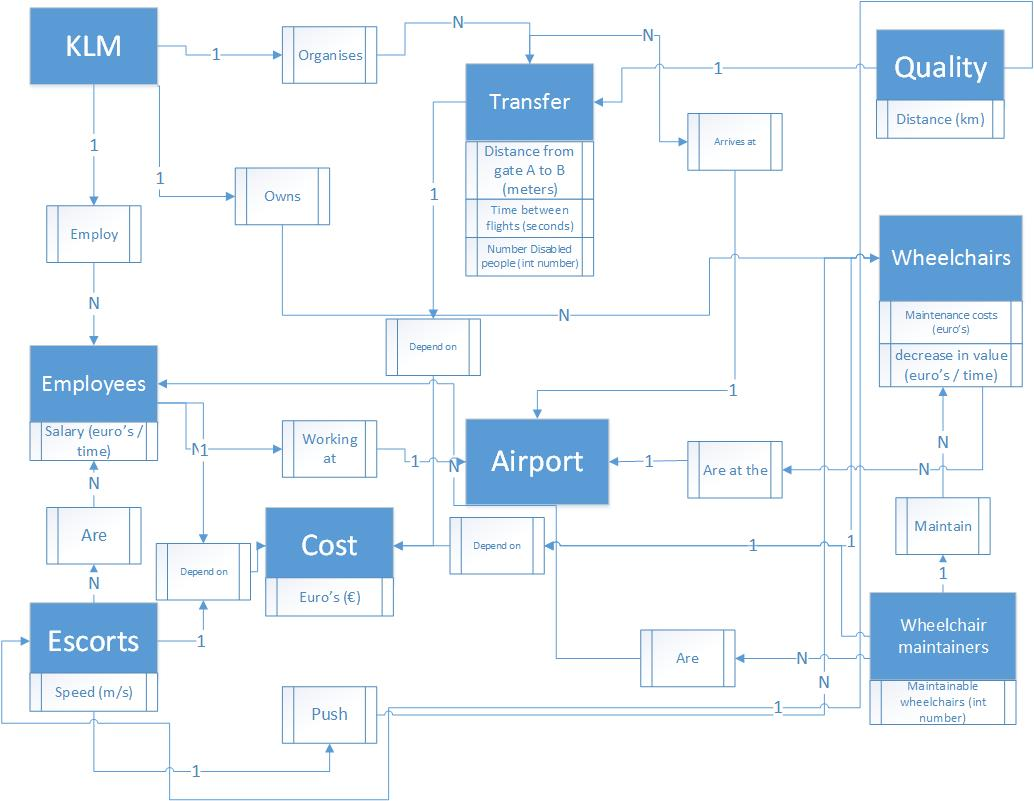
\includegraphics[scale=0.5]{figures/Conceptualmodel.jpg}
\clearpage
\section{Explanation of}
\subsubsection{KLM}
The "Money" property is the amount of money KLM has in this model.

\subsection{N on N relations of employees, escorts and maintainers}
These are very loose relations. In words this would be: some employees are escorts and some employees are maintainers.

\subsection{Time}
There are two values that are described in the unit "euro's/time". This time is not a predetermined value, because it is not known yet in what timeframe we would like to pay them.

\subsection{Money}
As one can see, all of the quantities are either usable to determine the eventual amount of money or are already quantified in money.


\setcounter{chapter}{+9}
\chapter{Quantities and their relationships}
	\section{Employees}
	\begin{description}
	\itemsep0em
	\item[Property:] Salary
	\item[Unit:] Euro's / hour
	\item[Role:] Constant\footnote{Average salary}  (Category 3)
	\end{description}
	\section{Transfer}
	\begin{description}
	\itemsep0em
	\item[Property:] Distance from gate A to B
	\item[Unit:] Meters
	\item[Role:] To be chosen  (Category 1)
	\end{description}
	\begin{description}
	\itemsep0em
	\item[Property:] Time between flights
	\item[Unit:] Seconds
	\item[Role:] To be chosen  (Category 1)
	\end{description}
	\begin{description}
	\itemsep0em
	\item[Property:] Disabled people
	\item[Unit:] An integer number
	\item[Role:] To be chosen  (Category 1)
	\end{description}
	\section{Escorts}
	\begin{description}
	\itemsep0em
	\item[Property:] Speed
	\item[Unit:] m/s
	\item[Role:] Constant (Category 3)
	\end{description}
	\section{Wheelchairs}
	\begin{description}
	\itemsep0em
	\item[Property:] Cost and maintenance cost
	\item[Unit:] Euros
	\item[Role:] Constant  (Category 3)

	\item[Property:] Decrease in value
	\item[Unit:] Euros/time
	\item[Role:] Constant (Category 3)
	\end{description}
	\section{Wheelchair maintainers}
	\begin{description}
	\itemsep0em
	\item[Property:] Wheelchairs they can maintain
	\item[Unit:] Integer
	\item[Role:] Constant  (Category 3)
	\end{description}

\chapter{Approximations and assumptions}

    \section{Approximations}
        \subsection{Speed of the escorts}
        In real life the escorts probably won't move at a constant speed. Making a turn it will be slower than walking in a straight line. How crowded it is at the airport also effects the walking speed, since you can't move at full speed when it is really crowded. However, to take all of this into account our actual model would be really hard. Therefore we let the escorts in our model move at a constant speed over a certain distance.

        \subsection{Distance between gates}
        The distance the escorts walk between the gates depends on the exact path they take. This path is different every time, because it depends on the number of people at the airport. On a busy day, the escorts have to go left and right to go around the people. This increases the travelled distance. This is impossible to keep in mind when creating the model. Therefore the distance between two gates is a constant value.

	\section{Assumptions}
		\subsection{Escort exhaustion} For the model the assumption holds that the escorts will never tire. This means that the morning hours of an escort are just as productive as his final hours. This assumption is necessary, because humans do not tire in the same way. There will be huge differences between escorts and these will be nearly impossible to calculate. There are scenarios in which the exhaustion rate of the escorts is nearly zero. For instance, the scenario with world-class athletes as escorts.
		
		\subsection{Infinite costs} When an airplane, in the real world, misses his timeslot, then the KLM will get fined. This fine is incredibly high. Moreover they will also be put on the blacklist. Meaning that the next time the plane arrives at an airport and there is a queue,then this plane will have to wait, at the cost of fuel and time. This second phenomena leads to the second assumption: the cost of missing the timeslot is infinite.
		
		\subsection{Other costs} This model's purpose is to estimate and optimize the costs for helping disabled people through their transfer. There is no need to implement other costs then that. The third assumption is that the model will be influenced by these costs and that the model does not influence those costs.
		
\chapter{Derivations}
	\section{Formulas}
\begin{description}
	\item $Costs = CostEscorts + CostMaintainers + CostMaintanance + CostDecrease$
	\item[Explanation:] These costs come from the conceptual model. They are all the costs.
	\item $CostEscorts = Salary * NrEscorts$
	\item $CostMaintainers = Salary * NrMaintainers$
	\item[Explanation:] This is basic economy. Total cost for a group of employees is, how many employees * their salary.
	\item $CostMaintanance = \frac{CostDecrease}{2} $ if it is more then this, you should seriously consider replacing it.
	\item[Explanation:] If the costs for repairing is more then half that it lost in value then most stores consider the vehicle total loss. Source: the garage that Yoram worked in.
	\item
	\item $Costs = Salary * NrEscorts + Salary * NrMaintainers + \frac{3* CostDecrease}{2}$
	\item[Explanation:] Substituted the cost functions in our main function.
	\item $TotalDistance = 2*distance*NrDisabled$
	\item[Explanation:] Total distance travelled by all the escorts to get all disabled people form their gate to the new gate.
	\item $TotalDistance1Escort = Vescort*TimeBetweenFlights$
	\item[Explanation:] This is basic kinematics. distance = average velocity.
	\item $NrEscorts = \frac{TotalDistance}{TotalDistance1Escort} = \frac{2*distance*NrDisabled}{(Vescort*TimeBetweenFlights)}$
	\item
	\item $NrMaintainers = \frac{NrWheelchairs}{WheelchairsPerMaintainer}$
	\item $NrWheelchairs = NrEscorts$
	\item[Explanation:] Because every escorts gets his own wheelchair, the number of wheelchairs are per definition equal to the number of escorts.
	\item $NrMaintainers = \frac{NrEscorts}{WheelchairsPerMaintainer}$
	\item
	\item $CostDecrease  = CostWheelchairPerSecond * TimeBetweenFlights * NrEscorts$
	\item[Explanation:] It takes time to get from one gate to another. Instead of calculation the decrease in value over days, we take the decrease in value in the time between the flights. So it is the decrease of one wheelchair in that time * the amount of wheelchairs.
	\item $CostWheelchairPerSecond = \frac{TotalCostWheelchair}{TimeTillDestruction}$
	\item[Explanation:] Assumed is that the decease in value is linear. This is allowed because CostWheelchairPerSecond is really small, so there would not be a really big difference and it is not far from the exact truth. TimeTillDestruction is the time until the wheelchairs are broken by use. All these values can be found on the internet.
	\item $CostDecrease  = TimeBetweenFlights * NrEscorts * \frac{TotalCostWheelchair}{TimeTillDestruction}$
	\item
	\item $Costs = Salary * NrEscorts + Salary * \frac{NrEscorts}{WheelchairsPerMaintainer} \\ \\+ \frac{3* TimeBetweenFlights * NrEscorts * TotalCostWheelchair}{2*TimeTillDestruction}$
	\item $Costs = NrEscorts * (Salary + \frac{Salary}{WheelchairsPerMaintainer} + \frac{3* TimeBetweenFlights * TotalCostWheelchair}{2*TimeTillDestruction}$
	\item $Costs = \frac{2*distance*NrDisabled}{(Vescort*TimeBetweenFlights)} * \\ \\(Salary + \frac{Salary}{WheelchairsPerMaintainer} + \frac{3* TimeBetweenFlights * TotalCostWheelchair}{2*TimeTillDestruction}$
	\item[Explanation:] Substitution gives us our final equation.
	\item
	%make purgy
\end{description}


\subsection{Domains}
	\begin{description}
		\item[Distance] $(0,\infty)$ The distance between the flights can be as large as we want it to be, but it cannot be infinite, negative or 0. This is because the domain or TimeBetweenFlights depends on this distance and cannot be zero. Thus if we exclude 0 from the domain of the distance we prevent a division by zero error in the domain of TimeBetweenFlights.
		\item[NrDisabled] $[0,853 ]$ The biggest passenger aircraft in the world, the Airbus A380 can fly 853 people. This becomes the upperbound to this domain, with zero disabled people as the lower bound.   %source: http://nl.wikipedia.org/wiki/Airbus_A380 oeps... wikipedia...
		\item[Vescort] $(0,3]$ 3m/s is a really fast military pace, which is possible for some people. There is not a physical possibility to walk $0m/s$, thus this is excluded from the domain, as well as all the negative numbers.
		\item[TimeBetweenFlights] First compute $\frac{2*distance}{Vescort} = c$ then the domain for the time becomes $(c,\infty)$ %dynamic domain.
		\item[Salary] $[0,\infty)$ Any non-negative number would do fine.
		\item[WheelchairsPerMaintainer] $(0,48)$ A typical reparation takes at least half an hour. Assuming that a maintainer works 24 hours a day. Then he can, at best, maintain 48 wheelchairs. Which is a good upper bound to this domain. This cannot be zero, because then we divide by zero.
		\item[TotalCostWheelchair] $(0,1000)$ Most normal wheelchairs are about $400$ euros, but sometimes a special model is needed. For example a larger wheelchair for fat people. so $1000$ is a nice upper bound on the cost of a wheelchair. They are never free of costs. %source?
		\item[TimeTillDestruction] $(0,\infty)$ Cannot be zero, because of the division by zero limitation. And it has to be positive. Thus this domain comes into existance.
	\end{description}
	
	
\subsection{Summary table}
\begin{table}[h]
\begin{tabular}{|l|l|l|}
\hline
Property                 & Unit     & Functions                                                          \\ \hline
Cost                      & \euro    & CostEscorts+CostMaintainers+CostMaintanance+\\CostDecrease   \\ \hline
CostEscorts              & \euro    & Salary * NrEscorts                                   \\ \hline
CostMaintainers          & \euro    & Salary *NrMaintainers                         \\ \hline
Salary                   & \euro    & SalaryPerHour * TimeBetweenFlights                          \\ \hline
NrEscorts                & -        & TotalDistance/TotalDistance1Escort                     \\ \hline
NrMaintainers            & -        & NrWheelchairs/WheelchairsPerMaintainer             \\ \hline
NrWheelchairs            & -        & NrEscorts                                            \\ \hline
CostMaintanance          & -        & CostDecrease/2                                   \\ \hline
TotalDistance            & m        & 2* distance *NrDisabled                        \\ \hline
TotalDistance1Escort     & m        & Vescort *TimeBetweenFlights                   \\ \hline
NrEscorts                & -        & TotalDistance/TotalDistance1Escort                       \\ \hline
CostDecrease             & \euro    & CostWheelchairPerHour*TimeBetweenFlights*NrEscorts \\ \hline
CostWheelchairPerHour    & \euro /h & TotalCostWheelchair/TimeTillDestruction     \\ \hline
                         &          &                                                                    \\ \hline
TotalCostWheelchair      & \euro    & Slider                                                             \\ \hline
TimeTillDestruction      & h        & Slider                                                             \\ \hline
WheelchairsPerMaintainer & -        & Slider                                                             \\ \hline
NrWheelchairs            & -        & Slider                                                             \\ \hline
TimeBetweenFlights       & h        & Slider                                                             \\ \hline
Vescort                  & km/h     & Slider                                                             \\ \hline
NrDisabled               & -        & Slider                                                             \\ \hline
Distance                 & km       & Slider                                                             \\ \hline
\end{tabular}
\end{table}
\chapter{Special cases}
\section{Employees and maintainers}
The salary is in euro's/hour. This means the more hours are being worked, the more the cost for the KLM will be. Except for when the people work for free. So that they are volunteers.\\
\begin{equation}
CostEmployed = Salary * NrEmployed
\end{equation}
If the extremes are evaluated, then taking the limit:
\begin{multline}
\lim_{Salary \rightarrow 0}CostEmployed = Salary * NrEmployed = \lim_{NrEmployed \rightarrow 0}CostEmployed \\ = Salary * NrEmployed = 0
\end{multline}
So by either having no escorts or maintainers and/or no salary, there will be no costs. However this also results in no service hence this situation is not desired. On the other hand taking the limit to infinity;
\begin{multline}
\lim_{Salary \rightarrow \infty} CostEmployed = Salary * NrEmployed = \lim_{NrEmployed \rightarrow 0} CostEmployed \\ = Salary * NrEmployed = \infty
\end{multline}
This is neither desired as result for the costs. Therefore neither the salary or the number of employed should be infinite or 0.
\begin{equation}
\lim_{WheelChairsPerMaintainer \rightarrow 0} NrMaintainers = \frac{NrWheelchairs}{WheelchairsPerMaintainer}
\end{equation}
\begin{equation}
= \lim_{NrMaintainers \rightarrow 0}NrMaintainers = \frac{NrWheelchairs}{WheelchairPerMaintainer} = 0
\end{equation}


\subsection{Employees are free}
In this case, escorts would be volunteers. People who like to work with disabled people could apply for the job and help the KLM by bringing disabled people from their plane to the correct other plane. If this would happen, more people could be hired as volunteer and this also means that people could stay and wait together with the disabled people. Do some games take them to a diner or anything else. It is a real thing to think about, because people sometimes like to work with those people. On the other hand those people do not have the same responsibilities as someone who is getting paid for the job. This could be a disadvantage, but if you have double the amount of people and they are willing to work kind of hard then this is definitely a good opportunity.
\subsection{No escorts}
If there are no escorts, no people can be brought to their gate. This means either no plane will leave in time or there are by coincidence no disabled people flying that day.
\subsection{Infinite escorts}
If there are infinite many escorts, that means it will cost the KLM lots of money, except if all those escorts are volunteers or if just a part of the escorts are volunteers. In either case probably every plane will leave in time, because if there are so many escorts, they can bring all the disabled persons to their gate.
\subsection{No wheelchair maintainers}
If there are no wheelchair maintainers, no wheelchair can be fixed and thus every time a wheelchair breaks down a new one should be bought.
\subsection{Infinite Wheelchair maintainers}
If there are infinite wheelchair maintainers, all wheelchairs that break down can and will be fixed in time and thus no wheelchair will bought new. This does make it really expensive for KLM because they have to pay for all the salaries.
\subsection{Productive working}
If the wheelchair maintainers are really productive they can fix 48 wheelchairs a day. This means less people will have to be employed.
\subsection{Not productive working}
If someone is not working productively, that means that he does not fix any wheelchairs. So you do not actually need them. it is a waste of money
\section{Transfer}
Transfer has a few formulas with it, for example distance between the gates, amount of disabled people who need to be transferred and the time between to flights. \\
So what happens when you find the limits of those, the most distant gate or the same gate, no disabled people or a plane full of disabled people and almost no transfer time or infinite or really long transfer time.\\
\begin{equation}
Totaldistance = 2 * distance *Nrdisabled
\end{equation}
\begin{equation}
Totaldistance1Escort= Vescort * TimeBetweenFlights
\end{equation}
\begin{equation}
\lim_{distance \rightarrow \infty} TotalDistance = 2 * distance * NrDisabled
\end{equation}
\begin{equation}
 = \lim_{NrDisabled \rightarrow \infty} TotalDistance = 2 * distance * NrDisabled = \infty
\end{equation}
\begin{equation}
\lim_{distance \rightarrow 0} TotalDistance = 2 * distance * NrDisabled
\end{equation}
\begin{equation}
= \lim_{NrDisabled \rightarrow 0} TotalDistance = 2 * distance * NrDisabled = 0
\end{equation}
\begin{equation}
\lim_{TimeBetweenDistance \rightarrow \infty} TotalDistance1Escort = Vescort*TimeBetweenFlights
\end{equation}
\begin{equation}
= \lim_{Vescort \rightarrow \infty} TotalDistance1Escort = Vescort*TimeBetweenEscort = \infty
\end{equation}
\begin{equation}
\lim_{TimeBetweenDistance \rightarrow 0} TotalDistance1Escort = Vescort*TimeBetweenFlights
\end{equation}
\begin{equation}
= \lim_{Vescort \rightarrow 0} TotalDistance1Escort = Vescort*TimeBetweenEscort = 0
\end{equation}

\subsection{Same gate}
The nearest gate to drop of someone is the gate he arrives at. This means the distance is zero so no distance, so no escort is needed to push him to his gate. Even if there are a hundred disabled people, even if it is a plane full of disabled people and you have 10 transfer seconds, you still do not need any escorts, because they already are at the place they need to be.
\subsection{furthest gate}
The gate which is most distant. If you only need to take one person there, you also only need one person to push him there. If there are multiple people who need to go to the most distant gate, you will need more people. It is only possible to push one person at a time for a escort. This means that if the plane is full of disabled people, you will need 853 escorts to push all those people to the same place. If the time in which this has to be done is really small and actually not realistic, only then it is allowed to prioritize other planes and let some people wait. There is no other reason why people should have to wait.
\subsection{No disabled people}
If there are no disabled people, no escorts are needed, so no extra money is involved in a flight.
\subsection{Plane full of disabled people}
A plane full of disabled people contains approximately 853 persons. All those persons need to be brought to the right gate. There are no mistakes allowed, else multiple planes might have a delay. So 853 escorts are needed to bring all those people to different or the same gate. If those people all need to go to different planes and some of those planes have a real high transfer time, then it is possible to use less escorts. So an escort could first take the people with an higher priority, which means that their plane leaves earlier. After they have brought the first person to their plane, they go back to the previous gate and pick up another person.
\section{wheelchairs}
Wheelchairs have two functions, one for the price and one for the devaluing of the wheelchair. What if a wheelchair is free or really expensive and what if they do not decrement or they are immediately worthless?\\
\begin{equation}
CostWheelchairs = Price * AmountOfWheelchairs
\end{equation}
\begin{equation}
CostWheelchairsPerSecond = \frac{TotalCostWheelchair}{TimeTillDestruction}
\end{equation}
\begin{equation}
CostDecrease = CostWheelchairPerSecond * TimeBetweenFlights * NrEscorts
\end{equation}
\begin{equation}
CostMaintenance = \frac{CostDecrease}{2}
\end{equation}
\subsection{Free}
If the wheelchairs are free, no wheelchair maintainers are needed. So wheelchairs will actually cost nothing.
\subsection{No decrement}
If the value of a wheelchair does not decrement, they can be sold for the same price as you have bought them. This also means that wheelchairs will never be broken too much. So they will live forever.
\subsection{immediately valueless}
If wheelchairs are immediately valueless after you have bought them, it is best to check the duration of a wheelchair and decide after that wether or not to buy a new wheelchair or fix the wheelchair.
\chapter{Estimates}
    \section{Speed of Escorts}
    The average walking speed of humans aged 14 to 64 is about 1.25 m/s  ($=$4.5 km/h). Since the escorts will have to take a wheelchair with them and it will be harder to move a wheelchair during rush hours the average speed of escorts will be estimated 1.19 m/s ($=$4.3 km/h).
    \section{Salary}
    According to \href{https://disabledaccessdenied.wordpress.com/2012/10/08/airport-wheelchair-fakes-are-making-life-hard-for-disabled-travellers/}{\emph{this (link)}} article the escorts earn something in between \$9 and \$14 an hour. So the estimated average would be \$11.50, which is about \euro{10.25}.\\
    According to \href{http://work.chron.com/average-wage-wheelchair-repair-19790.html}{\emph{this (link)}} article the average salary of wheelchair maintenance is \$23.99 an hour, this is about \euro{21.39}.\\
    Since there are way less wheelchair maintainers needed compared to escorts, the estimated salary will be \euro{12,-}.
    \section{New price for wheelchairs}
    New wheelchairs of acceptable quality are in a price range of \euro{275,-} to \euro{400,-}, more expensive would not be necessary, cheaper will bring the quality to low. Since there has to be a certain ratio between quality and cost: better quality results in happier customers, and probably less maintenance and a longer lifetime, however this would cause the costs to rise. The estimate of the cost of a wheelchair with a good quality/cost ratio is \euro{340,-}
    \section{Lifetime of a wheelchair}
    The average home use wheelchair which has a good and frequent maintenance schedule will be in service for about fifteen years. Since the wheelchairs at an airport are very intensively used it is reasonable to estimate the average lifetime of a airport wheelchair to be 7 years.
\setcounter{chapter}{+14}
\chapter{Rephrased problem in formal terms}

	\section{Formal definition of the problem}
	What will the minimal cost for KLM be and how many escorts, wheelchairs and wheelchair maintainers are needed for this to be achieved, given the distance between the gate of arrival and the gate of departure, the amount of time until the next flight leaves and the number of disabled people, while still getting all disabled people on board in time?
	
	\section{Explanation for the formal definition of the problem}
	The goal of the model is to have the total cost to be as small as possible, while still getting all disabled people on board in time. To achieve this, some other values need to be calculated first. Like:
\begin{itemize}
\itemsep0em
  \item How many escorts are needed?
  \item How many wheelchairs are needed?
  \item How many wheelchair maintainers are needed?
\end{itemize}
These values can be calculated from certain constants in the model and some values which have to be entered by the user of the model. These values are:
\begin{itemize}
\itemsep0em
  \item The distance between the gate of arrival and the gate of departure.
  \item The amount of time until the departing flight leaves.
  \item The number of disabled people.
\end{itemize}
Adding up all these things leads to the formal definition of the problem above.

%third deadline

\chapter{Calculation, implementation and simulation}
    Initially, we just put the formulas that are mentioned in the derivation into Accel. We used sliders for the values:
    \begin{itemize}
    \itemsep0em
    \item\vspace{-8pt} NrDisabled
    \item Distance
    \item Vescort
    \item TimeBetweenFlights
    \item WheelchairsPerMaintainer
    \item TotalCostWheelchair
    \item SalaryPerHour
    \item TimeTillDestructionPerYear
    \end{itemize}

<<<<<<< HEAD
\vspace{-8pt}These values can be adjusted by the KLM so they can see the cost associated with those values. But when trying to calculate the optimal values using Genetic Optimization, proposed inputs for the category one inputs as salary, number of disabled people and distance etc. are to be 0 to create minimal solutions. Some of them (\textbf{\textit{REFERENCE}}) have been made constant (so a category 3 property), in order to create a real life situation.
=======

These values can be adjusted by the KLM so they can see the cost associated with those values. But when trying to calculate the optimal values using Genetic Optimization, proposed inputs for the category one inputs as salary, number of disabled people and distance etc. are to be 0 to create minimal solutions. Some of them (NrDisabled, Distance, TimeBetweenFlights, WheelchairsPerMaintainer and SalaryPerHour) have been made constant (so a category 3 property), in order to create a real life situation.
>>>>>>> origin/master
To retrieve an optimized solution for the model, an extra category 2 property has been added as well as two pareto functions. This added property is the quality (defined by a Pareto function) and the added Pareto functions are:
=======
These values can be adjusted by the KLM so they can see the cost associated with those values. But when trying to calculate the optimal values using Genetic Optimization, proposed inputs for the category one inputs as salary, number of disabled people and distance etc. are to be 0 to create minimal solutions. Some of them (NrDisabled, Distance, TimeBetweenFlights, WheelchairsPerMaintainer and SalaryPerHour) have been made constant (so a category 3 property), in order to create a real life situation. To retrieve an optimized solution for the model, an extra category 2 property has been added as well as two pareto functions. This added property is the quality (defined by a Pareto function) and the added Pareto functions are:
>>>>>>> origin/master
\begin{center}
\vspace{-4pt}$Cost=paretoHor(paretoMin(CostEscorts+CostMaintainers+$\\$CostMaintenance+CostDecrease))$
\end{center}
\begin{center}
\vspace{-8pt}$Quality=paretoVer(paretoMax(max(0,10-NrDisabled/NrEscorts)))$
\end{center}
\vspace{-4pt}Before the solution of the Genetic Optimization is discussed, the following graphs retrieved from analyzing the model will be analyzed.
\begin{figure}[!h]
\caption{The cost of function of the costs of the escort personnel}
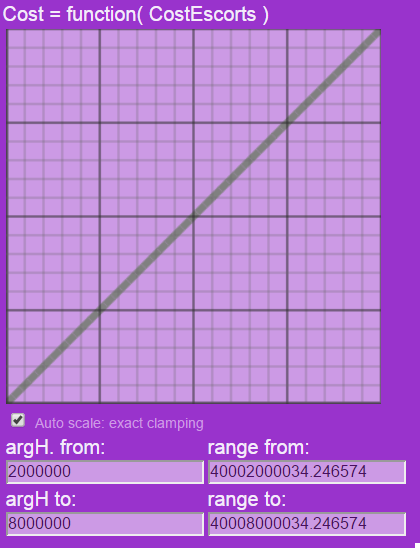
\includegraphics[width=0.3\textwidth]{figures/cost(CE)}
\caption{The cost of function of the time till the wheelchairs will be unusable}
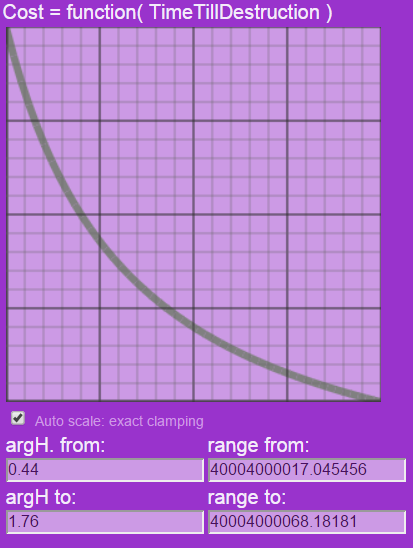
\includegraphics[width=0.3\textwidth]{figures/cost(TTD)}
\caption{The cost of function of the time between the flights}
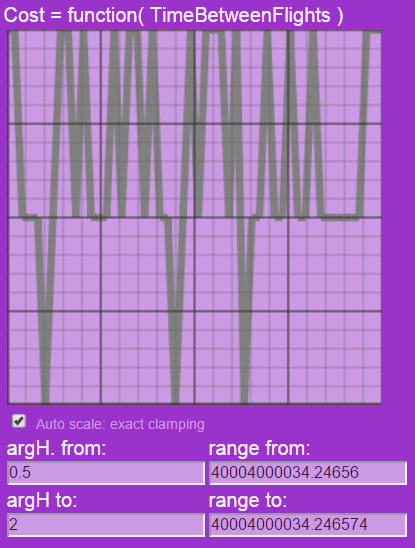
\includegraphics[width=0.3\textwidth]{figures/cost(TBF)}
\end{figure}
\\ \\
Figure 16.1 is a linear function, which follows from the formula for the cost, given by
>>>>>>> origin/master
\begin{equation}
Costs = CostEscorts + CostMaintainers + CostMaintanance + CostDecrease
\end{equation}
Assume that the other costs are constant, then there is a 1 to 1 correspondence from the costs to the cost of the cost of the personnel. Since CostEscort is also defined as a linear function (given by CostEscort = Salary $\cdot$ NrEscorts), the cost by function of the cost of the escort personnel should be linear. \\
Figure 16.2 contains a concave up line displaying the relation between the cost and the lifespan of a wheelchair. When analyzing this function by relating the cost to the property TimeTillDestruction:
\begin{equation}
CostDecrease = CostWheelchairPerSecond \cdot TimeBetweenFlights*NrEscorts
\end{equation}
\begin{equation}
CostWheelchairPerSecond= \frac{TotalCostWheelchair}{TimeTillDestruction}
\end{equation}
the following can be concluded. If CostDecrease in formula 16.1 is substituted by the above formulas, and the assumption is made that all other properties are constant, then the Cost is related to the TimeTillDestruction by:
\begin{equation}
Cost = \frac{c_1}{TimeTillDestruction}+ c_2
\end{equation}
where both $c_1$ and $c_2$ are constants. This shows that the relation is a fractional relation between the Cost and the TimeTillDesctruction which is in accordance to the concave up graph.\\

\chapter{Validation and verification; accuracy and precision}
We cannot get a ground value. This could be measured, but this is not within our power. Therefore we try a different approach to "proof" that our model is trustworthy. We first take a look at the dependencies. Then we take a look at the extremes, and see if this results in intuitive behaviour in our model. We also do a dimension analysis. We do not have convergence in our model, since we have no infinite series. This is therefore ignored. And we take a look at the conditional numbers.

\subsection{Dependencies} The network function of Accel shows us that the model has no cycles in it. Every cat 2 quantity is related the cat 1,2,3 quantities. The behaviour of all quantities are as expected, like you can see in the analysis section.

\subsection{Extremes} We look at 4 input variables:
	\subsubsection{Vescort} When this is near zero the cost explode. This is logical because we need a lot of escorts to bring all the people to the right place. When this speed goes near it upper bound, then we have a decrease in cost, since we can have multiple disabled people per escort. This decreases the quality of our service though. This behaviour is according to intuition.
	\subsubsection{WheelchairsPerMaintainer} The same inversely proportional behaviour exists for WheelchairsPerMaintainer. With little wheelchairs per maintainer we need a lot of maintainers, and thus have huge costs. This quantity does not influence quality.This is according to the reality. Because if wheelchairsPerMaintainer did influence the quality then the quality would decrease, because the wheelchairs are not maintained properly. So the maintainer cannot handle this amount of wheelchairs so then the number of wheelchairsPerMaintainer is wrong and should be decreased, which contradicts with the assumption that we could maintain them. So we conclude that this quantity should not influence the quality.
	\subsubsection{TotalCostWheelchair} When the wheelchairs cost more, then the costs become more... This is fairly obvious behaviour and according to reality.
	\subsubsection{TimeTillDestruction} This value does influence the costs, but only very very little. This is logical as well. If we have a lifetime of a wheelchair of, let say 5 years, then that 4 hour period that it is used during our flight will not cause a great increase in costs. This quantity is inversely proportional to the costs, when the lifetime of the wheelchairs go up, then the cost decrease, but only very little.
	
\subsection{Dimension analysis} Accel tells us that the dimension analysis is a go. We do this by checking the "check units" box and verify this with the units in the table in the formal model. These check out.

\subsection{Conditional numbers} We do a sensitivity analysis and we get the following conditional numbers:
\begin{description}
\item the first number relates to the costs and the second to the quality
	\item[Vescort]	0.50	0.0000025
	\item[WheelchairsPerMaintainer]		0.50	0.0
	\item[TotalCostWheelchair]		4.3e-10	0.0
	\item[TimeTillDestructionPerYear]		4.2e-10	0.0
	\end{description}
	We have no numbers over 1, this means that any uncertainty in the input will not correspond to a great uncertainty in the output.
	
\subsection{Conclusion} The model behaves intuitively and the uncertainty in the input does not correspond to a great uncertainty in the output. We therefore conclude that the model is precise, accurate to the problem and that it works like it should. We now have a verified and valid solution to the problem.
% \chapter{Conclusion phase}
% \section{Presentation and interpretation}

\chapter{Presentation and interpretation}
Our purpose is best served with a graph, because the model should give a value for multiple variables. Multiple variables can be chosen by the demanding company, in this case the KLM. those variables that can be chosen will lead to an output of the model, which is a graph. This is because there are multiple cases that lead to those equal variables.  \\ \\

It is actually a pretty precise model, of course we miss something, but it is all new for us so we are still learning. The things we miss are not of mature importance and can be implemented, but we think that such a thing is waste of time and money. They will cost more money to implement then they will make them. This means that the will not optimize the model enough to be of an actual value to the model and the company.
\setcounter{chapter}{+18}
\chapter{Discussion after the conceptual model}
\begin{enumerate}
    \item   Just like in the example we chose to leave out wind speed, because most of the time the escorts will be walking inside a building, this and knowing that wind does not really affect walking. Due to these two arguments we think wind speed might be left out.
    \item
\end{enumerate}

\chapter{Discussion after the conceptual model}
	\section{Stakeholders and keydrivers} In hindsight we picked the right stakeholders. But two of the have changed. These are the "Constuctors and maintainers of the wheelchairs" and "Other airline companies/airports". We choose to ignore the constructors, since their presence in the model is only in the cost of the wheelchair, a value later present in the maintenance costs of the wheelchair property.  And we ignored other airlines. This is because every flight gets allocated to a time in which it should leave, therefore not influencing other airlines. %source?
	
	\section{Optimization} We initially wanted to optimise both the cost and the time. We moved away from this idea because the time is fixed: we need to leave in x minutes. We then chose to optimise the cost and the quality of the product.
	
	\section{Conceptual model} The conceptual model has been updated after the meeting in the third week. We did not need all the original properties. We simply discarded them from the conceptual model. We only discarded those properties that are nearly impossible to quantify, which causes trouble in the formalization phase. Also we had the total cost of the wheelchair about three times in there, hidden in different properties.
	
<<<<<<< HEAD
	\section{Conclusion} Overall we think that we did a pretty good job for the conceptual model. It provided a solid basis for the formal model and it holds up with the stakeholders and keydrivers.
=======
	\section{Conclusion} Overall we think that we did a pretty good job for the conceptual model. It provided a solid basis for the formal model and it holds up with the stakeholders and keydrivers.

>>>>>>> origin/master
\chapter{Discussion after the formal model}
We have chosen to use a constant value for the values of NrDisabled, distance, TimeBetweenFlights and SalaryPerHour.\\
	
	\section{NrDisabled}
The number of disabled people on a flight is a constant for optimization purposes. If we optimize the model using accel the  model will always give a plane with zero disabled people as the optimal solution and because there is no control over this, we decided to make this a fixed number.
	
	\section{distance}
This also has to do with optimization, since the cost go down significantly if the distance between gates goes down without huge impact on the quality, and since there is no control over this (it is not possible to move gates closer together for a few minutes and then move them back) this should not be set to zero during optimization.
	
	\section{TimeBetweenFlights}
The time between flights is also not always possible to edit, so during optimization accel should not change this.
	
	\section{SalaryPerHour}
Ofcourse accel will try to put the salaries to zero since that would be the most cost efficient. This is not an acceptable outcome for the model. The salaries should be normal so these are made constant for optimization.

\chapter{Discussion after the result}

	\section{The graphs}
	
\chapter{Discussion after the solution of the initial problem}

\chapter{Extension}
If we had another week we would make the model more extensive and probably do more research, such that we know for sure that we have not forgotten anything. That means we really want to know wether or not we have found al variables that are on influence on the cost of an airport. With an extra week it would also be possible to check for importance of cost, priority. For example the cost of  salary is in comparison to the cost of a delayed plane not as much. This one we have already implemented in the report, but with an extra week we could check for more of these things. If we find more of those things our model gets more precise, which is really nice for the KLM.

\chapter{Necessity for Improvement}
We think our model needs to be improved on Convincingness. There are more things where the model can be improved, but on this aspect the model should actualy be improved.
\section{Convincingness}
There are special cases in our model which are not very likely to happend, it might not be really convincing to take these cases into account. On this point there is room for improvements.
\chapter{Possibilities for Improvement}
\section{Genericity}
    We think our overall view is quite big, which means that our case is a bit difficult, but less difficult case could also be applied. This means we do not think we have tot improve this.
\section{Scalability}
    Our model will always function, maybe not for a few special-cases like everybody in the world is disabled, which means there do not exist escorts. In this case ofcourse our model will not work. If you look to our model in a normal way, you will notice that it will always work, the difference will be the cost for the KLM in this case.
\section{Specialization}
    It is best to represent it in a graph, such that the problem owner easily can see what contributes to what.
\section{Audience}
    So because it is for the KLM, and to be more specific for the board of the KLM, we do not think it will be a big audience. Also we hope the audience has at least a little bit of knowledge of the basic subject. Because of all this we can implement more specialization. Also we can have more contact with the group such that we can skip subjects of the model, because they are already known, or we could stick longer to a subject to make it more clear.
\section{Convincingness}
    This might be one of the few parts which might be improved. We have made some assumptions in the special cases which are possible, but the probability is really low. So there might be a time where it will happen, but the current board of KLM will probably never experience something like this and for the next board the probability is also really low. So those assumptions are possible but not probable.
\section{distinctiveness}
    We tried to make a lot of variation between alternatives, sometimes really small variations, but we still think it is possible to improve some things.
\section{Surprise}
    There exist a lot of numbers which might not even exist in the future or that they depend on completely different things in the future. For now the numbers halt and it has an open outcome. In the future it will probably still be an open outcome, but the numbers might differ from what they are now. for example planes are a lot safer, and bigger. So more people will fly by plane and they might all fit in half of the planes we use now.
\section{Impact}
    This criteria is actually quite difficult, because a plane needs to be safe  the board of the KLM want to make as much profit as possible. This means there are two opposites involved. Either prestige and profit which needs more impact or risk and responsibility which needs less impact. So that is why you could always improve this criteria, because if you choose one the other will be neglected. which in either case will cost money.
	
\chapter{Aspects to be proud of}
	We think it is fair to say that there are a lot of aspects we are proud of. Of course the team is one of them, without our team and teamwork, we would have never been able to deliver such a product.
	
	\section{M. Ras}I will have to admit that it was an honor for me to work with these awesome guys. Sometimes it could be quite annoying, but after we actually started working and ignored the ones whom were annoying, they would start working and we could finish whatever it was we wanted to finish. So i would like to say that i am really proud of the teamwork. To just emphasize this, i would like to say that i am really proud of what we have achieved in the few weeks we have been working on this. I think it was an honor to make this report with these guys.
	
	\section{Y. Meijaard} I am very proud of the derivations and about the eventual model. I am proud of the conceptual model, it is very thorough and covers a lot of aspects. The eventual Accel model is fine, I would like to see a dynamical version of it. But this will take a few more months to get the quality that I want. And I am very proud of this group, although not every moment was productive, it was a honour working with these fine gentlemen.

\section{C. v. Horssen} I really like the result of eight weeks of work, I am proud on the final result. Also The teamwork was pretty good, everyone did his part of the project. It is a shame this project is already finished, we could have achieved so much more with our model if we would have more time.
\chapter{What have we learned?}
	\section{M. Ras}
	One of the favorite things i have learned is the modeling process itself. I really think it will be useful later on in my life and I also thought is was pretty fun to do so. The one and only thing I actually did not like about this course was making the model in accel. Before I started I had no idea what it should be able to do and know I know, I also know the program is not really nice to work with. It actually lags social skills if you would compare it to a human.
	
	\section{Y. Meijaard}
	I have learned a serious amount of mathematical tricks. I learned to extract the important pieces of a concept, quantify these and draw conclusions from their result. The moddelling procces is an useful skill, but I think that the to-do list method and Accel, although I learned how it works, will never again be useful.

\section{C. v. Horssen} During this course I have learned how github works, also I learned how the process of creating a model works and what you should take in mind while designing a model. There is some calculus with multiple variables in the course as well, this was new to me and I found this very interesting.
%%%%%%%%% INFORMATION %%%%%%%%%%
% \section{A Note About References}

% The Third and Fourth Year Handbook, and the Third and Fourth Year Project Handbook, have some clear guidelines about plagiarism and referencing.
% You should consult your project supervisor about the correct format for handling references.

% This document uses the `in-text' or Harvard system of referencing, which is a good default format.
% This requires both in-text citations and a list of references at the end of the document.
% The project templates have an example of a list of references.

% Within the text you must cite the authors surname(s) and the date of publication.
% When referring to a specific idea, or a direct quote, you must also give the page number.
% If there are two authors, use `and' and if there are more, use `et al.'\ and give all the authors names at the end.

% There are two styles of citation, implicit and explicit.
% Both are equally acceptable and it is also acceptable to mix and match.

% \subsubsection{Examples of implicit in-text citations}

% The sum of convex functions is itself convex (Blacke, 1985) and therefore any minimiser of this objective function will be a global minimiser (Greene and Whit, 1995, p.123). It is possible to exploit this fact (Browne et al., 2005) to enhance the optimisation algorithm.

% \subsubsection{Examples of explicit in-text citations}

% Blacke (1985) first proved that a sum of convex functions is convex. Any minimiser of this objective function will be a global minimiser, a fact shown by Greene and Whit (1995, p.123) and exploited by Browne et al.\ (2005) to enhance the optimisation algorithm.

%%%%%%%%% APPENDIX %%%%%%%%%%
% \appendix
% \chapter{An Appendix may not be necessary}

% Text introducing the/this appendix.

% \section{Appendix section}

% Text of this section.

% subsubsections and further divisions can also be used in appendices.

%%%%%%%%% BIBLIOGRAPHY %%%%%%%%%%
% \chapter*{Bibliography}

% \begin{description}

% \item Author, I. (Year). \emph{Book Title}, Publisher; Place of publication.

% \item Lamport, L. (1986), \emph{\LaTeX: A Document Preparation System}, Addison-Wesley; Reading, MA.

% \item Author, I. (Year). `Journal article title', \emph{Journal}, \textbf{Vol}, pp.first--last.

% \item Smith, A.D.A.C. and Wand, M.P. (2008). `Streamlined variance calculations for semiparametric
% mixed models', \emph{Statistics in Medicine}, \textbf{27}, pp.435--48.

% \end{description}

\end{document}
